%%  -*- ispell-local-dictionary: "american-w_accents" -*-
\documentclass[utf8x]{beamer}
\usepackage{etex}
\usepackage[english]{babel}
\usepackage[utf8x]{inputenc}
\usepackage[T1]{fontenc}
\usepackage{amsmath,amsthm,amsfonts}
\usepackage[all, color, pdf]{xy}
\usepackage{mathtools}
\usepackage{xcolor}
%\usepackage{realboxes} % for \Colorbox
\usepackage{skull} % for \skull
%\usepackage{ulem}
\usepackage{marvosym} % for \Lightning
\usepackage{amssymb}
\usepackage{cancel}
\usepackage{fourier} % for \danger
\usepackage{tikz}
\usetikzlibrary{arrows, decorations.pathmorphing, decorations.pathreplacing,
  decorations.markings, decorations.text, positioning, shapes.geometric,
  arrows.meta, backgrounds, fit, math}
  %arrows.meta, backgrounds, fit, math,shapes,calc
%\usepackage{manfnt}
\usepackage[scaled=0.85]{beramono}
\renewcommand{\ttdefault}{pcr}
\usepackage{listings}
\usepackage{lstcoq}
\lstset{language=Coq}
%\lstset{backgroundcolor=\color{black!15}}
%\lstset{basicstyle=\scriptsize\bf\ttfamily,escapeinside={(*@}{@*)}}
\usepackage{annotate}
\definecolor{idee}{rgb}{1,0,1}
\usepackage{boxedlistings}
\lstset{style=script}

\lstset{escapeinside={(*@}{@*)}}

\pgfdeclareimage[height=10mm]{robot}{figures/R2D2-small.jpeg}
\pgfdeclareimage[width=.4cm]{jumelles}{figures/jumelles.jpg}
\pgfdeclareimage[width=.4cm]{calculette}{figures/calculette.jpg}
\pgfdeclareimage[width=.4cm]{deplacement}{figures/deplacement.jpg}
\pgfdeclareimage[width=.7\textwidth]{the-end}{figures/the-end.pdf}
\newcommand{\jum}{\raisebox{-.1cm}{\pgfuseimage{jumelles}}}
\newcommand{\calc}{\raisebox{-.1cm}{\pgfuseimage{calculette}}}
\newcommand{\dep}{\raisebox{-.1cm}{\pgfuseimage{deplacement}}}
\pgfdeclareimage[width=.5cm]{jumelles'}{figures/jumelles.jpg}
\pgfdeclareimage[width=.5cm]{calculette'}{figures/calculette.jpg}
\pgfdeclareimage[width=.5cm]{deplacement'}{figures/deplacement.jpg}
\newcommand{\bjum}{\raisebox{-.1cm}{\pgfuseimage{jumelles'}}}
\newcommand{\bcalc}{\raisebox{-.1cm}{\pgfuseimage{calculette'}}}
\newcommand{\bdep}{\raisebox{-.1cm}{\pgfuseimage{deplacement'}}}

%\usecolortheme{crane}


\setbeamertemplate{navigation symbols}{}
\setbeamercovered{invisible}

\definecolor{mygreen}{rgb}{0,.6,0}
\newcommand\hfilll{\hskip 0pt plus 1filll}
\newcommand\cit[1]{\hfill {\scriptsize \textcolor{purple}{[#1]}}}
\newcommand\gris[1]{\uncover{{\color{gray} #1}}}
\newcommand\auteur[2]{#1~\textsc{#2}}
\newcommand\mycite[1]{\textcolor{purple}{#1}}
\newcommand\Checkmark{\textcolor{mygreen}{\checkmark}}
\newcommand<>{\alertb}[1]{\alt#2{\textcolor{blue}{#1}}{#1}}

% Rising dots
\makeatletter
\def\revddots{\mathinner{\mkern1mu\raise\p@
\vbox{\kern7\p@\hbox{.}}\mkern2mu
\raise4\p@\hbox{.}\mkern2mu\raise7\p@\hbox{.}\mkern1mu}}
\makeatother

\tikzset{robot/.pic={\draw[fill=red] (0,0) circle [radius=.1, draw=black] {};}}
\tikzset{robotA/.pic={\draw[pic actions] (0,0) circle [radius=.1, draw=black];}}
\tikzset{ref/.pic={\draw[->] (0,0) -- (0,0.5); \draw[->] (0,0) -- (0.5,0);}}
\tikzset{cross/.pic={\draw[color=blue] (-0.1,0) -- (0.1,0) (0,-0.1) -- (0,0.1);}}
\definecolor{gentil}{rgb}{.5,.5,.9}
\tikzstyle{rond}=[circle=1pt,draw=black]
\newcommand{\robot}[3]{\node (r) at (#1,#2) [draw,color=#3,fill,rond] {};}
\newcommand{\drawrobotonly}[5]{
  \begin{scope}[xshift=#3,yshift=#4,scale=#1,rotate=#2]
    \robot{0}{0}{#5}
  \end{scope}
}
\newcommand{\drawrobot}{\drawrobotonly}

\usetikzlibrary{arrows,chains,calc}

\title{Formal Proofs for Mobile Robot Swarms}
\author{\auteur{Lionel}{Rieg}}
\institute{Ensimag -- Grenoble INP / VERIMAG}
\date[2 avril 2019]{Réunion Estate/Descartes, Roscoff, 2 avril 2019}


\begin{document}

\frame{\maketitle}


\section{Motivations}
%%%%%%%%%%%%%%%%%%%%%

\begin{frame}
  \frametitle{Inspiration: Swarms of Mobile Robots}

    \includegraphics<2>[width=\linewidth, keepaspectratio]{figures/alice-micro-robot-swarm}
    \includegraphics<3>[width=\linewidth, keepaspectratio]{figures/kilobot-swarm}
    \includegraphics<6>[width=\linewidth, keepaspectratio]{figures/JO-intel}
    \includegraphics<7>[width=\linewidth, keepaspectratio]{figures/navy}

    \only<1,4-5,8->{
      \begin{itemize}
        \item Swarms?
          \pause \pause \pause
          \begin{itemize}
            \item lots of (small) identical robots
          \end{itemize}
          \pause \vspace{1em}
        \item Where?
          \pause \pause \pause
          \begin{itemize}
            \item entertainment
            \item rescue
            \item exploration
%%             \item industry 4.0
            \item \dots
          \end{itemize}
          \pause \vspace{1em}
        \item Opportunities?
          \begin{itemize}
            \item cooperative behavior (swarm intelligence)
            \item resilience
          \end{itemize}
          \vspace{1em}
        \item Main challenge?
          \begin{itemize}
            \item Understand what happens!
          \end{itemize}

      \end{itemize}
    }
\end{frame}

\begin{frame}
  \frametitle{Why Formal Methods for Mobile Robots Swarms?}

  \alert{Many} mobile robots swarm models:
  \begin{itemize}
    \item \alert<2>{Space} \hfill
      \gris{\small discrete/continuous, bounded/unbounded, topology, \dots}
    \item \alert<3>{Sensors} \hfill
      \gris{\small multiplicity, range, accuracy, orientation, \dots}
    \item \alert<4>{Faults} \hfill
      \gris{\small none, crash, Byzantine, \dots}
    \item \alert<5>{Execution} \hfill
      \gris{\small synchronous/asynchronous, fairness, interruption, \dots}
  \end{itemize}
  \pause \bigskip

  \begin{overlayarea}{\linewidth}{11.4em}
    \only<2,3,4>{
      \vspace{2em}
      \begin{center}
        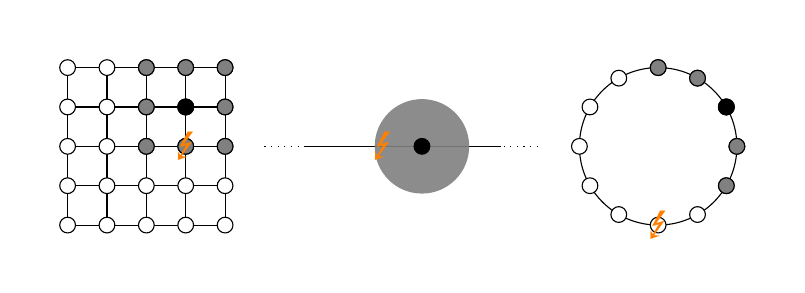
\begin{tikzpicture}
          % frame
          \draw[transparent] (0.5,0.5) rectangle (10,3.5);
          % spaces
          % -- grid
          \draw[step=0.5cm] (0.99,0.99) grid (3,3); % .99 = rounding errors
          \foreach \a in {1, 1.5, ..., 3}
            \foreach \b in {1, 1.5, ..., 3}
              \draw[fill=white] (\a,\b) circle [radius=0.1cm];
          % -- line
          \draw[style=dotted] (3.5,2) -- (7,2);
          \draw (4,2) -- (6.5,2);
          % -- ring
          \draw (8.5, 2) circle [radius=1cm];
          \foreach \a in {0, 30, ..., 330}
            \draw[fill=white] (8.5,2) + (\a:1cm) circle [radius=0.1cm];
          % ranges
          \foreach \x in {-0.5, 0, 0.5} \foreach \y in {-0.5, 0, 0.5}
            \draw<3>[fill=gray] (2.5,2.5) + (\x,\y) circle [radius=0.1cm];
          \draw<3>[fill] (2.5,2.5) circle [radius=0.1cm];
          \fill<3>[fill=gray,fill opacity=0.9] (5.5,2) circle [radius=0.6cm];
          \draw<3>[fill] (5.5,2) circle [radius=0.1cm];
          \foreach \a in {-30, 0, ..., 90}
            \draw<3>[fill=gray] (8.5,2) + (\a:1cm) circle [radius=0.1cm];
          \draw<3>[fill] (8.5,2) + (30:1cm) circle [radius=0.1cm];
          % faults
          \node<4> at (2.5,2.5) {\small \textcolor{red}{$\skull$}};
          \node<4> at (2.5,2) {\Large \textcolor{orange}{\Lightning}};
          \node<4> at (5.5,2) {\small \textcolor{red}{$\skull$}};
          \node<4> at (5,2) {\Large \textcolor{orange}{\Lightning}};
          \node<4> at (9.36,2.5) {\small \textcolor{red}{$\skull$}};
          \node<4> at (8.5,1) {\Large \textcolor{orange}{\Lightning}};
        \end{tikzpicture}
      \end{center}
    }
    \only<5>{
      % FSYNC
      \begin{minipage}{.48\linewidth}
        \tiny
        \begin{tabular}{|@{}c@{}|@{}c@{}|@{}c@{}|@{}c@{}|}
          Round 1 & Round 2 & Round 3 & Round 4 \\[.5em]
          \jum\calc\dep&\jum\calc\dep & \jum\calc\dep& \jum\calc\dep \\
          \jum\calc\dep&\jum\calc\dep & \jum\calc\dep& \jum\calc\dep \\
          \jum\calc\dep&\jum\calc\dep & \jum\calc\dep& \jum\calc\dep \\
          \jum\calc\dep&\jum\calc\dep & \jum\calc\dep& \jum\calc\dep \\
        \end{tabular}
      \end{minipage} \hfill
      % SSYNC
      \begin{minipage}{.48\linewidth}
        \tiny
        \begin{tabular}{|@{}c@{}|@{}c@{}|@{}c@{}|@{}c@{}|}
          Round 1 & Round 2 & Round 3 & Round 4 \\[.5em]
          \jum\calc\dep& & \jum\calc\dep& \jum\calc\dep \\
          \jum\calc\dep& \jum\calc\dep& &  \\
          & \jum\calc\dep&\jum\calc\dep& \jum\calc\dep\\
          \jum\calc\dep& & & \jum\calc\dep \\
        \end{tabular}
      \end{minipage} \vspace{.5em}

      % ASYNC
      ~\hfill
        \begin{minipage}{.78\linewidth}
          \tiny \vspace{1em}
          \begin{tabular}{|p{2cm}|c|c|c|c|c|c|c@{\,}} \hline
            & \centering \jum & {\calc} & \dep& \jum& \calc & \dep &
            $\cdots$ \\ \hline
          \end{tabular}
          \begin{tabular}{|p{.7cm}|p{3.25cm}|p{1.3cm}|p{0.9cm}}\hline
            \centering \jum& \centering\calc& \centering\dep & $\cdots$ \\ \hline
          \end{tabular}
          \begin{tabular}{|p{5.15cm}|c|c|p{0.2cm}}\hline
            \centering \jum & \centering \calc & \centering \dep &
            $\cdots$\\ \hline
          \end{tabular}
          \begin{tabular}{|c|c|c|c|c|c|c|c|p{0.82cm}}\hline
            \jum & \calc & \dep & \jum & \calc & \dep & \jum & \calc & ~~\dep \\ \hline
          \end{tabular}
        \end{minipage}
      \hfill~
    }
    \only<6->{
      \begin{minipage}{0.09\linewidth}
        \alert{\Huge \danger}
      \end{minipage}
      \begin{minipage}{0.88\linewidth}
        \begin{itemize}
          \item \alert{Subtle differences} in models $\leadsto$ \alert{Very} error-prone
          \item Careful of mismatch spec/proof!
          \item Lots of proof cases
        \end{itemize}
      \end{minipage}
      \medskip

      $\Rightarrow$ Formal methods can help

      \pause \pause \pause \pause \pause \bigskip
      Which model? (process algebra, TLA, \dots) \\
      Which tool? (model checking, proof assistant, \dots) \\
      \bigskip
      \alert{We need a suitable framework}
      \hfill \gris{\small What are the requirements?}
    }
  \end{overlayarea}
\end{frame}


\section{Overview of the Model}
%%%%%%%%%%%%%%%%%%%%%%%%%%%%%%%

\begin{frame}
  \frametitle{Robot Model \hfilll \small [Suzuki, Yamashita 99]}

  \begin{itemize}
    \item<2-> Points
    \item<3-> With Byzantine faults (or crash)
    \item<4-> Anonymous
    \item<5-> No direct communication
    \item<6-> No common frame/direction \\
      $\leadsto$ \alert{local} coordinates
    \item<7-> Limited/unlimited vision? multiplicity?
    \item<8-> \alert{Same} (deterministic) program everywhere
  \end{itemize}
  \begin{center}
    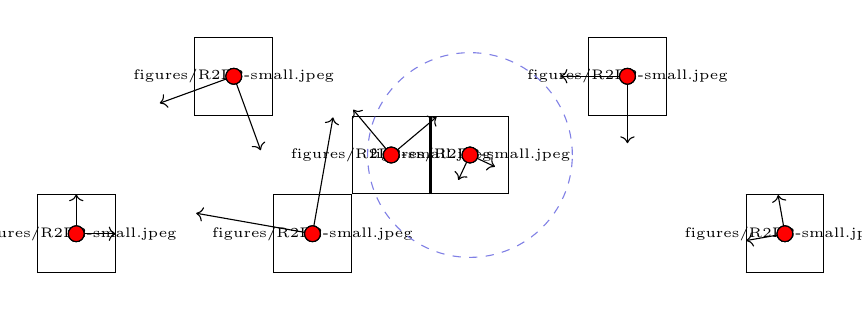
\begin{tikzpicture}
      % frame
      \draw (0,0.7) (0,3.5);
      % pictures of robots
      \node<1> at (0,1) {\pgfuseimage{robot}};
      \node<1> at (3,1) {\pgfuseimage{robot}};
      \node<1> at (5,2) {\pgfuseimage{robot}};
      \node<1> at (4,2) {\pgfuseimage{robot}};
      \node<1> at (2,3) {\pgfuseimage{robot}};
      \node<1> at (9,1) {\pgfuseimage{robot}};
      \node<1> at (7,3) {\pgfuseimage{robot}};
      % Dots for robots
      \pic<2>[fill=gentil] at (0,1) {robotA};
      \pic<2>[fill=gentil] at (3,1) {robotA};
      \pic<2>[fill=gentil] at (5,2) {robotA};
      \pic<2>[fill=gentil] at (4,2) {robotA};
      \pic<2>[fill=gentil] at (2,3) {robotA};
      \pic<2>[fill=gentil] at (9,1) {robotA};
      \pic<2>[fill=gentil] at (7,3) {robotA};
      % With Byzantine faults
      \pic<3>[fill=gentil] at (0,1) {robotA};
      \pic<3>[fill=orange] at (3,1) {robotA};
      \pic<3>[fill=gentil] at (5,2) {robotA};
      \pic<3>[fill=orange] at (4,2) {robotA};
      \pic<3>[fill=gentil] at (2,3) {robotA};
      \pic<3>[fill=gentil] at (9,1) {robotA};
      \pic<3>[fill=orange] at (7,3) {robotA};
      % Orientation
      \pic<6> at (0,1) {ref};
      \pic<6>[rotate=80,scale=3] at (3,1) {ref};
      \pic<6>[rotate=245,scale=0.7] at (5,2) {ref};
      \pic<6>[rotate=40,scale=1.5] at (4,2) {ref};
      \pic<6>[rotate=200,scale=2] at (2,3) {ref};
      \pic<6>[rotate=100] at (9,1) {ref};
      \pic<6>[scale=1.7,rotate=180] at (7,3) {ref};
      % Final robots dots
      \pic<4-> at (0,1) {robot};
      \pic<4-> at (3,1) {robot};
      \pic<4-> at (5,2) {robot};
      \pic<4-> at (4,2) {robot};
      \pic<4-> at (2,3) {robot};
      \pic<4-> at (9,1) {robot};
      \pic<4-> at (7,3) {robot};
      % Limited visibility
      \draw<7>[color=gentil, dashed] (5,2) circle [radius=1.3];
    \end{tikzpicture}
  \end{center}
  % TODO: dessins en overlay pour les 4 propriétés au dessus?
\end{frame}


\begin{frame}
  \frametitle{Execution Models (1) \hfilll \small [Suzuki, Yamashita 99]}

  3 phases for each robot:
  \begin{enumerate}
    \item \bjum \; \alert{Look}: observe its surrounding \\
      \begin{itemize}
        \item indirect communication 
        \item depends on sensor capabilities
      \end{itemize} \medskip
    \item \bcalc \; \alert{Compute}: choose what to do
      \begin{itemize}
        \item choose an objective
        \item depends on observation, program
      \end{itemize} \medskip
    \item \bdep \; \alert{Move}: do it (or try to)
      \begin{itemize}
        \item try to reach your target
        \item depends on the environment
      \end{itemize}
  \end{enumerate}
  \pause
  \alert{and repeat}
\end{frame}

\begin{frame}
  \frametitle{Execution Models (2): Scheduling \hfilll \small [Suzuki, Yamashita 99]}

  Scheduling of robots is
  \begin{itemize}
    \item[Either]<2->\alertb{ASYNC}: full interleaving \\
      \begin{itemize}
        \item<2-> Most general/realistic but hardest
      \end{itemize}
    \item[or]<3-> Same phase for all active robots
      \begin{itemize}
        \item<3-> Time split into rounds
        \item<4-> \alertb{FSYNC}: \alert{all} robots are activated each round
        \item<5-> \alertb{SSYNC}: only a \alert{subset} is activated \\
          $\leadsto$ \alert{Fairness} assumptions on the scheduling (demon)
      \end{itemize}
  \end{itemize}
  \bigskip

  \hspace{1.5cm}
  \begin{overlayarea}{0.7\linewidth}{3cm}
    % ASYNC
    \only<2>{
    \vspace{.5em}
      \begin{tabular}{|p{2cm}|c|c|c|c|c|c|c@{\,}} \hline
        & \centering \bjum & {\bcalc} & \bdep & \bjum & \bcalc & \bdep &
        $\cdots$ \\ \hline
      \end{tabular}
      \begin{tabular}{|p{.7cm}|p{3.25cm}|p{1.3cm}|p{0.9cm}}\hline
        \centering \bjum & \centering\bcalc & \centering\bdep & $\cdots$ \\ \hline
      \end{tabular}
      \begin{tabular}{|p{5.15cm}|c|c|p{0.2cm}}\hline
        \centering \bjum & \centering \bcalc & \centering \bdep &
        $\cdots$\\ \hline
      \end{tabular}
      \begin{tabular}{|c|c|c|c|c|c|c|c|p{0.82cm}}\hline
        \bjum & \bcalc & \bdep & \bjum & \bcalc & \bdep & \bjum & \bcalc & ~~\bdep \\ \hline
      \end{tabular}
    }
    % just Rounds
    \only<3>{
      \begin{tabular}{|@{}c@{}|@{}c@{}|@{}c@{}|@{}c@{}|@{}c@{}|}
        Round 1 & Round 2 & Round 3 & Round 4 & Round 5 \\[.5em]
        \phantom{\bjum\bcalc\bdep} &
        \phantom{\bjum\bcalc\bdep} &
        \phantom{\bjum\bcalc\bdep} &
        \phantom{\bjum\bcalc\bdep} &
        \phantom{\bjum\bcalc\bdep} \\
         & & & & \\
         & & & & \\
         & & & & \\
      \end{tabular}
    }
    % FSYNC
    \only<4>{
      \begin{tabular}{|@{}c@{}|@{}c@{}|@{}c@{}|@{}c@{}|@{}c@{}|}
        Round 1 & Round 2 & Round 3 & Round 4 & Round 5 \\[.5em]
        \bjum\bcalc\bdep & \bjum\bcalc\bdep & \bjum\bcalc\bdep & \bjum\bcalc\bdep & \bjum\bcalc\bdep \\
        \bjum\bcalc\bdep & \bjum\bcalc\bdep & \bjum\bcalc\bdep & \bjum\bcalc\bdep & \bjum\bcalc\bdep \\
        \bjum\bcalc\bdep & \bjum\bcalc\bdep & \bjum\bcalc\bdep & \bjum\bcalc\bdep & \bjum\bcalc\bdep \\
        \bjum\bcalc\bdep & \bjum\bcalc\bdep & \bjum\bcalc\bdep & \bjum\bcalc\bdep & \bjum\bcalc\bdep \\
      \end{tabular}
    }
    % SSYNC
    \only<5>{
      \begin{tabular}{|@{}c@{}|@{}c@{}|@{}c@{}|@{}c@{}|@{}c@{}|}
        Round 1 & Round 2 & Round 3 & Round 4 & Round 5 \\[.5em]
        \bjum\bcalc\bdep & & \bjum\bcalc\bdep & \bjum\bcalc\bdep & \bjum\bcalc\bdep \\
        \bjum\bcalc\bdep & \bjum\bcalc\bdep & &  & \bjum\bcalc\bdep \\
        & \bjum\bcalc\bdep & \bjum\bcalc\bdep & \bjum\bcalc\bdep & \\
        \bjum\bcalc\bdep & & & \bjum\bcalc\bdep & \\
      \end{tabular}
    }
  \end{overlayarea}
\end{frame}


\section{Pactole approach}


\begin{frame}{fragile}\frametitle{\only<1-2>{Proving Distributed Protocol}
    \only<3->{Pactole}}
  \vfill
  \vfill
  \hfill
  \begin{minipage}{.95\linewidth}    
  \begin{tikzpicture}[x=0.5cm,y=0.5cm]
    \node(hg) at (-13,10){};
    \node(hg) at (6,-6){};
    \node[rectangle,draw] (model) at (-5,9) {\tikz\coordinate(modeltxt);Model};
    \node[rectangle,draw] (problem) at (-5,7) {\tikz\coordinate(probtxt);problem $\mathcal{P}$ + protocol $p$};
    \node[rectangle,draw] (inst) at (0,3.5) {instance(s) of $\mathcal{P}$};
    %\node[rectangle,draw] (Arect) at (0,0.5) {algorithm \tikz\coordinate(A);$A$};
    \node[rectangle,draw] (formul) at (0,0.5) { \tikz\coordinate(phi);$\Gamma\vdash_{LTL}\phi$?};
    \node[rectangle,draw] (proof) at (-10,2) {\tikz\coordinate(prooftxt);Direct proof};
    \node[rectangle,draw] (mc) at (0,-2.5) {MC};
    \draw[->] (inst) to (formul);
    \draw[->] (formul) to (mc);
    \draw[->] (model) to (problem);
    \draw[->] (problem) to (inst);
    \draw[->] (problem) to (proof);
    \annotate<2>[.25\linewidth]{width("fGLTLx")}{phi}{8em}{-1em}{true iff $p$ succeeds on all schedulings};      
    \annotate<3->{width("Modi")}{modeltxt}{12em}{0em}{Coq};      
    \annotate<3->{width("protocolxPxprotocolexp")}{probtxt}{12em}{0em}{Coq};      
    \annotate<3->{width("directproof")}{prooftxt}{6em}{0em}{Coq};      
    \coordinate [left=1cm of mc] (mcleft);
    \coordinate [right=1cm of mc] (mcright);
    \draw<4>[purple,-,ultra thick,opacity=.6](inst.north west) to (mcright);
    \draw<4>[purple,-,ultra thick,opacity=.6](inst.north east) to (mcleft);
  \end{tikzpicture}
  \end{minipage}
\vfill
  % \begin{overlayarea}{1.0\linewidth}{5em}
  %   \begin{onlyenv}<4>
  %   \begin{itemize}
  %   \item Why not prove $A$ in Coq?
  %   \item Needs: distributed model (reusable), protocol $p$, desrired
  %     properties of $p$, LTL formulas and semantics (reusable), $A$
  %     itself, proof of $A$
  %   \end{itemize}
  % \end{onlyenv}
  % \end{overlayarea}
\end{frame}


\section{The Pactole Formalization}
%%%%%%%%%%%%%%%%%%%%%%%%%%%%%%%%%%%

\begin{frame}<1,2>[label=pactole]
  \frametitle{Pactole: a Coq Framework for Mobile Robots}

  \alert{Very Parametric} (but still useful):
  \begin{itemize}
    \item Space
    \item State of Robots (\alert{location}, memory, battery level, etc.)
    \item Sensors
    \item How states are updated during the move phase
  \end{itemize}
  \bigskip

  \alert{Key Ingredients}:
  \begin{itemize}
    \item Configuration \hfill \gris{function ident $\to$ state}
    \item Spectrum \hfill \gris{info on config from sensors}
    \item Robogram \hfill \gris{function spectrum $\to$ location}
    \item Demon (scheduler) \hfill \gris{adversarial environment}
    \item \alert<2>{Round} \hfill \gris{one step of execution}
  \end{itemize}
\end{frame}

\begin{frame}
  \frametitle{Description of a Round}

  \alert{Robogram}: what happens for a robot?
  \begin{enumerate}
    \item<2-> If it is not activated, some update happens (for ASYNC only)
    \item<4-> If it is activated and Byzantine, the demon gives its new state
    \item<6-> If it is activated and not Byzantine (i.e. Good),
      \begin{enumerate}[a.]
        \item \textbf{Look}: get information from its surrounding
        \item \textbf{Compute} its destination
        \item \textbf{Move} to the destination
      \end{enumerate}
  \end{enumerate}
  \bigskip

  \alert{Demon}: what does the environment decide?
  \begin{enumerate}
    \item<3-> Pick which robots are activated
    \item<3-> Decide how to update inactive ones
    \item<5-> Update Byzantine ones as it wishes
    \item<7-> Select the new frame of reference for non Byzantine ones
    \item<7-> Decide how to update them depending on their destination
  \end{enumerate}
\end{frame}

\begin{frame}[fragile]
  \frametitle{The Core of Pactole: the Round Function}

  \begin{overlayarea}{\linewidth}{25 em}
  \scriptsize
  \begin{onlyenv}<1>
    \begin{lstlistingCoq}[emptylines=*50]
Definition round (r:robogram) (da:demonic_action) cfg
 : configuration :=
 fun id =>(*@\hfill@*)(* for a given robot, we compute the new state *)









 










     $\quad$
    \end{lstlistingCoq}
  \end{onlyenv}
  \begin{onlyenv}<2>
    \begin{lstlistingCoq}
Definition round (r:robogram) (da:demonic_action) cfg
 : configuration :=
 fun id =>(*@\hfill@*)(* for a given robot, we compute the new state *)
  if da.(activate) id(*@\hfill@*)(* see whether the robot is activated *)
  then




    


        
          

          

          



          

  else inactive cfg id (da.(choose_inactive) cfg id).
\end{lstlistingCoq}
  \end{onlyenv}
  \begin{onlyenv}<3>
    \begin{lstlistingCoq}
Definition round (r:robogram) (da:demonic_action) cfg
 : configuration :=
 fun id =>(*@\hfill@*)(* for a given robot, we compute the new state *)
  if da.(activate) id(*@\hfill@*)(* see whether the robot is activated *)
  then
   match id with
   | Byz b => da.(relocate_byz) cfg b(*@\hfill@*)(* byzantine *)
   | Good g =>



   


   
     

     



     
   end
  else inactive cfg id (da.(choose_inactive) cfg id).
\end{lstlistingCoq}
  \end{onlyenv}
  \begin{onlyenv}<4>
    \begin{lstlistingCoq}
Definition round (r:robogram) (da:demonic_action) cfg
 : configuration :=
 fun id =>(*@\hfill@*)(* for a given robot, we compute the new state *)
  if da.(activate) id(*@\hfill@*)(* see whether the robot is activated *)
  then
   match id with
   | Byz b => da.(relocate_byz) cfg b(*@\hfill@*)(* byzantine *)
   | Good g =>
     (* change the frame of reference *)
     let new_frame := frame_choice (da.(change_frame) cfg g) in
     let local_cfg := map_cfg (lift new_frame ( ... )) cfg in
     let local_pos := get_location (local_cfg (Good g)) in

     

     
     
     



     
   end
  else inactive cfg id (da.(choose_inactive) cfg id).
\end{lstlistingCoq}
  \end{onlyenv}
  \begin{onlyenv}<5>
    \begin{lstlistingCoq}
Definition round (r:robogram) (da:demonic_action) cfg
 : configuration :=
 fun id =>(*@\hfill@*)(* for a given robot, we compute the new state *)
  if da.(activate) id(*@\hfill@*)(* see whether the robot is activated *)
  then
   match id with
   | Byz b => da.(relocate_byz) cfg b(*@\hfill@*)(* byzantine *)
   | Good g =>
     (* change the frame of reference *)
     let new_frame := frame_choice (da.(change_frame) cfg g) in
     let local_cfg := map_cfg (lift new_frame ( ... )) cfg in
     let local_pos := get_location (local_cfg (Good g)) in
     (* compute the spectrum *)
     let spect := spect_from_cfg local_cfg local_pos in

     

     



     
   end
  else inactive cfg id (da.(choose_inactive) cfg id).
\end{lstlistingCoq}
  \end{onlyenv}
  \begin{onlyenv}<6>
    \begin{lstlistingCoq}
Definition round (r:robogram) (da:demonic_action) cfg
 : configuration :=
 fun id =>(*@\hfill@*)(* for a given robot, we compute the new state *)
  if da.(activate) id(*@\hfill@*)(* see whether the robot is activated *)
  then
   match id with
   | Byz b => da.(relocate_byz) cfg b(*@\hfill@*)(* byzantine *)
   | Good g =>
     (* change the frame of reference *)
     let new_frame := frame_choice (da.(change_frame) cfg g) in
     let local_cfg := map_cfg (lift new_frame ( ... )) cfg in
     let local_pos := get_location (local_cfg (Good g)) in
     (* compute the spectrum *)
     let spect := spect_from_cfg local_cfg local_pos in
     (* apply r on spectrum *)
     let local_traj := r spect in

     



     
   end
  else inactive cfg id (da.(choose_inactive) cfg id).
\end{lstlistingCoq}
  \end{onlyenv}
  \begin{onlyenv}<7>
    \begin{lstlistingCoq}
Definition round (r:robogram) (da:demonic_action) cfg
 : configuration :=
 fun id =>(*@\hfill@*)(* for a given robot, we compute the new state *)
  if da.(activate) id(*@\hfill@*)(* see whether the robot is activated *)
  then
   match id with
   | Byz b => da.(relocate_byz) cfg b(*@\hfill@*)(* byzantine *)
   | Good g =>
     (* change the frame of reference *)
     let new_frame := frame_choice (da.(change_frame) cfg g) in
     let local_cfg := map_cfg (lift new_frame ( ... )) cfg in
     let local_pos := get_location (local_cfg (Good g)) in
     (* compute the spectrum *)
     let spect := spect_from_cfg local_cfg local_pos in
     (* apply r on spectrum *)
     let local_traj := r spect in
     (* return to the global frame of reference *)
     let global_traj := lift_path (new_frame (*@\raisebox{-.3ex}{$^{-1}$}@*)) local_traj in



     
   end
  else inactive cfg id (da.(choose_inactive) cfg id).
\end{lstlistingCoq}
  \end{onlyenv}
  \begin{onlyenv}<8>
    \begin{lstlistingCoq}
Definition round (r:robogram) (da:demonic_action) cfg
 : configuration :=
 fun id =>(*@\hfill@*)(* for a given robot, we compute the new state *)
  if da.(activate) id(*@\hfill@*)(* see whether the robot is activated *)
  then
   match id with
   | Byz b => da.(relocate_byz) cfg b(*@\hfill@*)(* byzantine *)
   | Good g =>
     (* change the frame of reference *)
     let new_frame := frame_choice (da.(change_frame) cfg g) in
     let local_cfg := map_cfg (lift new_frame ( ... )) cfg in
     let local_pos := get_location (local_cfg (Good g)) in
     (* compute the spectrum *)
     let spect := spect_from_cfg local_cfg local_pos in
     (* apply r on spectrum *)
     let local_traj := r spect in
     (* return to the global frame of reference *)
     let global_traj := lift_path (new_frame (*@\raisebox{-.3ex}{$^{-1}$}@*)) local_traj in
     (* the demon chooses how to perform the state update *)
     let choice := da.(choose_update) cfg g global_traj in


   end
  else inactive cfg id (da.(choose_inactive) cfg id).
\end{lstlistingCoq}
  \end{onlyenv}
  \begin{onlyenv}<9>
    \begin{lstlistingCoq}
Definition round (r:robogram) (da:demonic_action) cfg
 : configuration :=
 fun id =>(*@\hfill@*)(* for a given robot, we compute the new state *)
  if da.(activate) id(*@\hfill@*)(* see whether the robot is activated *)
  then
   match id with
   | Byz b => da.(relocate_byz) cfg b(*@\hfill@*)(* byzantine *)
   | Good g =>
     (* change the frame of reference *)
     let new_frame := frame_choice (da.(change_frame) cfg g) in
     let local_cfg := map_cfg (lift new_frame ( ... )) cfg in
     let local_pos := get_location (local_cfg (Good g)) in
     (* compute the spectrum *)
     let spect := spect_from_cfg local_cfg local_pos in
     (* apply r on spectrum *)
     let local_traj := r spect in
     (* return to the global frame of reference *)
     let global_traj := lift_path (new_frame (*@\raisebox{-.3ex}{$^{-1}$}@*)) local_traj in
     (* the demon chooses how to perform the state update *)
     let choice := da.(choose_update) cfg g global_traj in
     (* actual state update performed by the update function *)
     update cfg g global_traj choice
   end
  else inactive cfg id (da.(choose_inactive) cfg id).
    \end{lstlistingCoq}
  \end{onlyenv}
  \end{overlayarea}
\end{frame}

\begin{frame}<1-3>[label=scheme]
  \frametitle{Proving in Pactole}

  \textbf{Correctness proof:}
  \begin{enumerate}
    \item<1-> Formalize your problem
    \item<2-> Write your robogram
    \item<3-> Express your algorithm in the global frame of reference \\
      \uncover<4->{Use geometric patterns that are \alert{invariant by change of frame} \\
        \hfill {\footnotesize
          \lstinlineCoq{Lemma round_simplify :  $\forall$ da cfg, round r da cfg == ...}}\hfill ~}
    \item<5-> Prove that your algorithm solves your problem \\
      following your paper proof
  \end{enumerate}
  \bigskip

  \uncover<6->{\textbf{Impossibility proof:}
  \begin{enumerate}
    \item Formalize your problem
    \item Assume given a robogram (a variable) + its properties
    \item Prove that the algorithm does not solve the problem \\
      (\lstinlineCoqv!round_simplify! not always needed)
  \end{enumerate}}
\end{frame}

\begin{frame}
  \frametitle{Two different points of view}

  \begin{tabular}{l|l}
    \textbf{Global View} (demon + proof) & \textbf{Local View} (robots) \\
    \hline
    absolute location & local frame of reference \\
    robots: Byzantine or not (B / G) & indistinguishable robots \\
    identifiers ident $= G + B$ \\
    configuration = ident → position
    & local configuration \\
    & spectrum \\
    & robogram \\
    & \hspace{1em} : spectrum → location \\
    round r d : config → config \\
    exec = stream of configurations \\
  \end{tabular}
  \bigskip

  spectrum = degraded local view of a configuration
\end{frame}


\againframe<3->{scheme}


\begin{frame}
  \frametitle{Some results (\Checkmark verified in Pactole)}

  \begin{itemize}
  \item Convergence $\mathbb{R}^2$, rigid, $\geq 1/3$ Byzantine, SSYNC \\
    \textcolor{red}{Impossibility}
    \hfill [Bouzid et al. TCS'10] \! \mycite{[SSS'13]} \Checkmark
  \item Gathering $\mathbb{R}^2$, rigid, no Byzantine, SSYNC \\
    \textcolor{red}{Impossibility} ($2\times n$ robots) \hfill
    [Suzuki,Yamashita SICOMP'99]\\
    \hfill \mycite{[IPL'15]} \Checkmark
  \item Gathering $\mathbb{R}^2$, rigid, no Byzantine,
    SSYNC, \alert{start not bivalent}\\
    \textcolor{mygreen}{Effective (universal) algorithm}\hfill \mycite{[DISC'16]}
    \Checkmark
  \item Gathering $\mathbb{R}^2$, \alert{non rigid}, no Byzantine, FSYNC, \alert{no
    multiplicity}\\
    \textcolor{mygreen}{Effective (universal) algorithm}
    \hfill \mycite{[SSS'16]} \Checkmark
    \item Exploration $\mathbb{Z}/n\mathbb{Z}$, \alert{discrete},  $k$ robots, no bizantine, SSYNC \\
    \textcolor{red}{Impossibility} ($k$ divides $n$) \hfill \mycite{[ICDCN'17]} \Checkmark
    \item \alert{Discrete/continuous graphs}, non rigid, ASYNC \\
      \textcolor{mygreen}{Model equivalence} \hfill \mycite{[SSS'18]} \Checkmark
    \item Connection $\mathbb{R}^2$, rigid, no bizantine, SSYNC \\
    \textcolor{mygreen}{Effective (non optimal) algorithm}\hfill \mycite{[SSS'21]} \Checkmark
  \end{itemize}
\end{frame}

\section{Gathering}
%%%%%%%%%%%%%%%%%%%

\begin{frame}[fragile]
  \frametitle{Case Study: Gathering}

  \begin{block}{Objective}
    Have all (non byzantine) robots reach in finite time the same location (unknown ahead of time) and then stay there.
  \end{block}
  \bigskip

  Let's formalize it!
  \pause

  \small
  \begin{lstlistingCoq}
(* All good robots are at the same location [pt] (exactly). *)
Definition gathered_at (pt : location) (cfg : configuration) :=
  $\forall$ g, get_location (cfg (Good g)) == pt.

(* At all rounds of [e], robots are gathered at [pt]. *)
Definition Gather (pt : location) (e : execution) : Prop :=
  Stream.forever (Stream.instant (gathered_at pt)) e.

(* The infinite execution [e] is *eventually* [Gather]ed. *)
Definition WillGather (pt : location) (e : execution) : Prop :=
  Stream.eventually (Gather pt) e.
  \end{lstlistingCoq}
\end{frame}


\begin{frame}
  \frametitle{Impossibility Proof \hspace{6em} [Suzuki \& Yamashita 99]}

  \begin{center}
    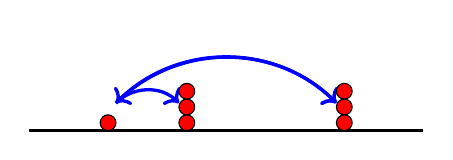
\begin{tikzpicture}
      % situation
      \draw (0,1.3);
      \draw[color=black, very thick] (0,0) -- (5,0);
      \pic<1-4> at (1,.1) {robot};
      \pic at (4,.1) {robot};

      % first case
      \draw<2>[color=blue, very thick, ->, bend left=45] (1.1,.35) to (3.9,.35);
      \draw<3>[color=blue, very thick, <->, bend left=45] (1.1,.35) to (3.9,.35);

      % second case
      \draw<4>[color=blue, very thick, ->, bend left=45] (1.1,.35) to (1.9,.35);
      \pic<5-> at (2,.1) {robot};

      % Several robots
      \pic<7> at (4,.3) {robot};
      \pic<7> at (4,.5) {robot};
      \pic<7> at (2,.3) {robot};
      \pic<7> at (2,.5) {robot};
    \end{tikzpicture}
  \end{center}

  By symmetry, both robots act the same. \\
  \medskip

  Two cases:
  \begin{enumerate}
    \item<2-3,6-> Left robot moves to the right one \\
      \uncover<3,6->{activate both: \alert<3>{swap locations}}
    \item<4-> Left robot goes anywhere else \\
      \uncover<5->{activate only the left one: \alert<5>{same configuration up to scale}}
  \end{enumerate}
  \pause \pause \pause \pause \pause
  In both cases, a \alert{similar configuration} at the next round
  \bigskip \pause

  Generalizations:
  \begin{itemize}
    \item Even number of robots
    \item Type of line ($ℚ$ ou $ℝ$), higher dimension
  \end{itemize}
\end{frame}

\begin{frame}
  \frametitle{Universal Algorithm}

  \alert{Key Ideas}:
  \begin{itemize}
    \item Center of the smallest enclosing circle
    \item Move in stages (not all robots at once)
      \item Never create the configuraton of the impossibility proof
  \end{itemize}
  \medskip

  Hard part of the proof: \alert{termination}
  \hfill $\leadsto$ \alert{termination order}
  \begin{itemize}
    \item \#robots on the circle decreases
    \item Stages
    \item Avoid looping with triangles
  \end{itemize}
  \pause

  \centering
  \scalebox{.74}{
  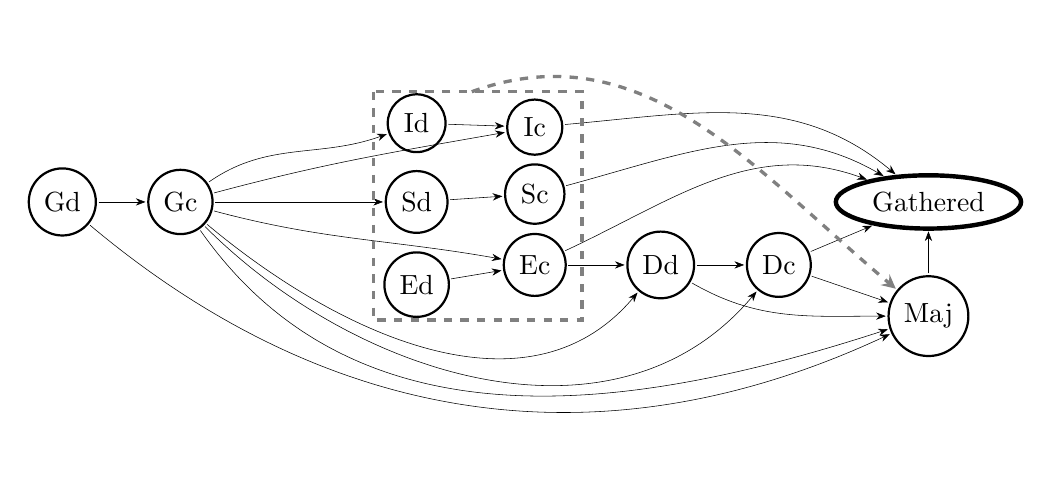
\begin{tikzpicture}[thick,>={Stealth[length=3.5pt]},outer sep = 1pt]
    \node (n) at (12,-0.4) [color=black,shape=ellipse,ultra thick,draw] {Gathered}; %
    \node (n0) at (12,-1.85) [shape=circle,draw] {Maj}; %
    \node (n1) at (10.1,-1.2) [color=black,shape=circle,draw] {Dc}; %
    \node (n2) at (8.6,-1.2) [color=black,shape=circle,draw] {Dd}; %
    \node (n3s) at (7,-0.3) [shape=circle,draw] {Sc}; %
    \node (n3i) at (7,0.55) [color=black,shape=circle,draw] {Ic}; %
    \node (n3e) at (7,-1.2) [shape=circle,draw] {Ec}; %
    \node (n4s) at (5.5,-0.4) [color=black,shape=circle,draw] {Sd}; %
    \node (n4i) at (5.5,0.6) [shape=circle,draw] {Id}; %
    \node (n4e) at (5.5,-1.45) [shape=circle,draw] {Ed}; %
    \node (n5) at (2.5,-0.4) [shape=circle,draw] {Gc}; %
    \node (n6) at (1,-0.4) [shape=circle,draw] {Gd}; %
    
    %%%% arcs
    \draw [color=black,line width=.2pt,->] (n0) to (n); %
    \draw [line width=.2pt,->] (n1) to (n); %
    \draw [color=black,line width=.2pt,->] (n2) to (n1); %
    \draw [color=black,line width=.2pt,->] (n3e) to (n2); %
    \draw [color=black,line width=.2pt,->,out=25,in=-200] (n3e) to (n); %
    \draw [color=black,line width=.2pt,->] (n4e) to (n3e); %
    \draw [color=black,line width=.2pt,->] (n4s) to (n3s); %
    \draw [color=black,line width=.2pt,->] (n4i) to (n3i); %
    \draw [color=black,line width=.2pt,->,out=5,in=140] (n3i) to (n); %
    \draw [color=black,line width=.2pt,->,out=15, in=-210] (n3s) to (n); %
    \draw [color=black,line width=.2pt,->,out=-15,in=-190] (n5) to (n3e); %
    \draw [color=black,line width=.2pt,->,out=15,in=-170] (n5) to (n3i); %
    \draw [color=black,line width=.2pt,->,out=-40,in=-130] (n5) to (n2); %
    \draw [color=black,line width=.2pt,->,out=-45,in=-130] (n5) to (n1); %
    \draw [color=black,line width=.2pt,->,out=35, in=200] (n5) to (n4i); %
    \draw [color=black,line width=.2pt,->,out=0,in=180] (n5) to (n4s); %
    \draw [color=black,line width=.2pt,->] (n6) to (n5); %

    \draw [color=black!50,->,>=stealth,out=20,in=140,dashed,very thick] (6.2,1) to (n0); %
    \draw [color=black,line width=.2pt,->,out=-40, in=-155] (n6) to (n0); %
    \draw [color=black,line width=.2pt,->,out=-30, in=-180] (n2) to (n0); %
    \draw [color=black,line width=.2pt,->,out=-55, in=-162] (n5) to (n0); %
    \draw [color=black,line width=.2pt,->] (n1) to (n0); %

    %%%% cadre
    \draw [color=black!50,dashed,very thick] (4.95,1) rectangle (7.6,-1.9);
  \end{tikzpicture}}
\end{frame}

\begin{frame}[fragile] \frametitle{Termination Order in Coq}
\begin{lstlistingCoq}
Definition m_clean s := nG-s[target s].
Definition m_dirty s := nG-SECT_cardinal s.
Function measure (s : observation): nat * nat :=
 match support (max s) with
 | nil => (0, 0)(*@\hfill@*)(* no robot *)
 | pt :: nil => (0, nG -  s[pt]) (*@\hfill@*)(* majority *)
 | _ :: _ :: _ =>
   match on_SEC (support s) with
   | nil | _::nil => (0,0) (*@\hfill@*)(* impossible cases *)
   | pt1::pt2::nil => (*@\hfill@*)(* diameter case *)
     if clean s then (1,m_clean s) else (2,m_dirty s)
   | pt1::pt2::pt3::nil => (*@\hfill@*)(* triangle case *)
     if clean s then (3,m_clean s) else (4,m_dirty s)
   | _ => (*@\hfill@*)(* general case *)
     if clean s then (5,m_clean s) else (6,m_dirty s)
 end
end.

Definition lt_config x y :=
(*@\hfill@*) Lexprod.lexprod lt lt (measure (!! x)) (measure (!! y)).
\end{lstlistingCoq}
\end{frame}


\begin{frame}\frametitle{Conclusion About Pactole}
  \begin{description}[\textcolor{mygreen}{\huge $\oplus$}]
    \item[\textcolor{mygreen}{\huge $\oplus$}] Designed for mobile robot swarms \\
      \uncover<2->{
        \begin{itemize}
          \item \bjum \, \bcalc \, \bdep\, cycle built-in
          \item Other features are possible
            \hfill \gris{\small memory, battery, \dots}
        \end{itemize}
      }
    \item[\textcolor{mygreen}{\huge $\oplus$}] Ease of use for specification
      \uncover<3->{
        \begin{itemize}
          \item Expressive logic (Coq)
          \item Maths can be directly expressed
          \item Principled bottom-up approach
        \end{itemize}
      }
    \item[\textcolor{mygreen}{\huge $\oplus$}] Broadly applicable \\
      \uncover<4->{
        \begin{itemize}
          \item Highly parametric \hfill
            \gris{\small space, sensors, execution model, \dots}
          \item Very expressive
          \item Common base of definition (no more mismatches)
        \end{itemize}
        $\Rightarrow$ A junction point for several formal results?
      }
    \item[\textcolor{red}{\huge $\ominus$}]<5> Caveat
      \begin{itemize}
        \item No fully automated procedure (yet)
        \item Building proofs is a lot of work
      \end{itemize}
  \end{description}
\end{frame}


\begin{frame} \frametitle{Future}
  \begin{itemize}
  \item ANR SAPPORO (2019-2023):
    \begin{itemize}
    \item Randomized protocols
    \item Automated proofs (graph rewriting)
    \item Non euclidean geometry (non-perfect sensors)
    \item Luminous robots
    \end{itemize}
  \item Link with model checkers
  \end{itemize}
\end{frame}

\begin{frame}
  \frametitle{Appendix: Link with model checking}
  \vfill
  \vfill
  \hfill
  \begin{minipage}{.95\linewidth}    
  \begin{tikzpicture}[x=0.5cm,y=0.5cm]
    \node(hg) at (-13,10){};
    \node(hg) at (6,-6){};
    \node[rectangle,draw] (model) at (-5,9) {\tikz\coordinate(modeltxt);Model};
    \node[rectangle,draw] (problem) at (-5,7) {\tikz\coordinate(probtxt);problem $\mathcal{P}$ + protocol $p$};
    \node[rectangle,draw] (inst) at (0,3.5) {\tikz\coordinate(insttxt);instance(s) of $\mathcal{P}$};
    \node[rectangle,draw] (Arect) at (0,0.5) {algorithm \tikz\coordinate(A);$A$};
    \node[rectangle,draw] (formul) at (0,-2.5) {LTL formula \tikz\coordinate(phi);$\phi$};
    \node[rectangle,draw] (proof) at (-10,0) {\tikz\coordinate(prooftxt);Direct proof};
    \node[rectangle,draw] (mc) at (0,-5) {MC};
    \draw[->] (inst) to (Arect);
    \draw[->] (Arect) to (formul);
    \draw[->] (formul) to (mc);
    \draw[->] (model) to (problem);
    \draw[->] (problem) to (inst);
    \draw[->] (problem) to (proof);
    \annotate[.25\linewidth]{width("f")}{phi}{6em}{-1em}{s.t. $\phi$ valid iff protocol succeeds on all schedulings};      
    \annotate<2->[.25\linewidth]{width("f")}{A}{6em}{1em}{by correctness of $A$ \alt<3->{\xcancel{(paper)}({\color{idee}Coq?})}{(paper)}};      
    \annotate<3->{width("instancexsxofP")}{insttxt}{6em}{0em}{Coq?};      
    \annotate{width("Modi")}{modeltxt}{12em}{0em}{Coq};      
    \annotate{width("protocolxPxprotocolexp")}{probtxt}{12em}{0em}{Coq};      
    \annotate{width("directproof")}{prooftxt}{6em}{0em}{Coq};      
  \end{tikzpicture}
  \end{minipage}
\vfill
  % \begin{overlayarea}{1.0\linewidth}{5em}
  %   \begin{onlyenv}<4>
  %   \begin{itemize}
  %   \item Why not prove $A$ in Coq?
  %   \item Needs: distributed model (reusable), protocol $p$, desired
  %     properties of $p$, LTL formulas and semantics (reusable), $A$
  %     itself, proof of $A$
  %   \end{itemize}
  % \end{onlyenv}
  % \end{overlayarea}
\end{frame}

\end{document}

%%% Local Variables:
%%% mode: latex
%%% TeX-master: t
%%% End:
